\documentclass[margin=3mm]{standalone}
\usepackage{tikz}
\begin{document}
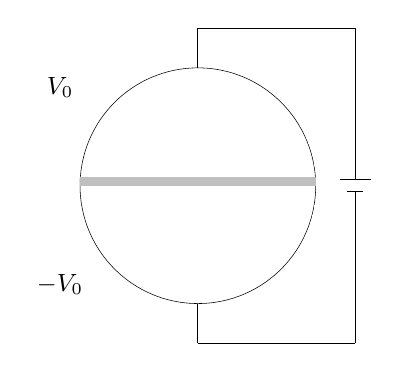
\begin{tikzpicture}[font=\small]
    \coordinate (A) at (0, 1.5);
    \coordinate (B) at (0, 2);
    \coordinate (C) at (2, 2);
    \coordinate (D) at (0, -1.5);
    \coordinate (E) at (0, -2);
    \coordinate (F) at (2, -2);


    \begin{scope}
        \clip (0,0) circle (1.5);
        \draw (0,0) circle (1.5);
        \draw [draw=black, fill,  color=gray!50] (-1.5, 0) rectangle (1.5, 0.1);
    \end{scope}

    \draw (A) -- (B);
    \draw (B) -- (C);
    \draw (D) -- (E);
    \draw (E) -- (F);
    \draw (C) -- (2, 0.075);
    \draw (F) -- (2, -0.075);
    \draw (1.8, 0.075) -- (2.2, 0.075);
    \draw (1.9, -0.075) -- (2.1, -0.075);
    
    \node at (-1.75, 1.25) {$V_{0}$};
    \node at (-1.75, -1.25) {$-V_{0}$};
\end{tikzpicture}
\end{document}